\documentclass{beamer}

\usepackage[ngerman]{babel}
\usepackage{lmodern}
\usepackage{mathtools}
\usepackage{amssymb}
\usepackage{tikz}
\usepackage{graphicx}
\usepackage{tabularx}
\usepackage{listings}
\usepackage{color}
\usetikzlibrary{shapes,decorations.pathreplacing,angles,quotes}
\usetheme{metropolis}
\setbeamertemplate{section in toc}[sections numbered]
%\setbeamertemplate{subsection in toc}[subsections numbered]

\definecolor{dkgreen}{rgb}{0,0.6,0}
\definecolor{gray}{rgb}{0.5,0.5,0.5}
\definecolor{mauve}{rgb}{0.58,0,0.82}

\lstset{frame=tb,
  language=Java,
  aboveskip=3mm,
  belowskip=3mm,
  showstringspaces=false,
  columns=flexible,
  basicstyle={\tiny\ttfamily},
  numbers=none,
  numberstyle=\tiny\color{gray},
  keywordstyle=\color{blue},
  commentstyle=\color{dkgreen},
  stringstyle=\color{mauve},
  breaklines=true,
  breakatwhitespace=true,
  tabsize=3
}

% Presentation metadata
\title{Analyzing Big Data Streams}
\author{Florian Kalinke}
\date{18. Dezember 2017}

\begin{document}

\maketitle

\begin{frame}[t]{Übersicht}
  \vspace*{0.5cm}
  \renewcommand{\baselinestretch}{0.75}\normalsize
  \tableofcontents
  \renewcommand{\baselinestretch}{1.0}\normalsize
\end{frame}


\section{Stream-Verarbeitung}

\subsection{Einsatzgebiete}
\begin{frame}[t]{Einsatzgebiete}
  \begin{itemize}
    \item Analyse von Sensordaten
    \item IoT Devices
    \item Fraud-Detection
    \item Complex Event Processing
    \item High Speed Trading Systeme
    \item Klickstream-Analyse

    \item \textit{Echtzeitsysteme}
  \end{itemize}
\end{frame}

\subsection{The Big Picture}
\begin{frame}[t]{The Big Picture}
  \begin{figure}
    \centering
    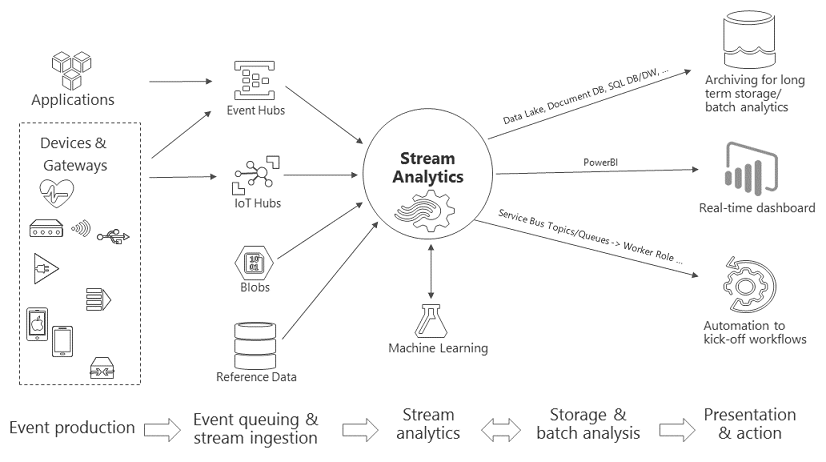
\includegraphics[scale=0.4]{img/stream_analytics_intro_pipeline.png}
    \caption{Übersicht einer Stream-Analyse Plattform\hspace{\linewidth} Bild von https://docs.microsoft.com/de-de/azure/stream-analytics/stream-analytics-introduction }
  \end{figure}
\end{frame}


\subsection{Abgrenzung zur Batch-Verarbeitung}

\begin{frame}[t]{Abgrenzung zur Batch-Verarbeitung}
  Ausschlaggebend für die Batch-Verarbeitung:
  \begin{itemize}
    \item Die Größe der Daten ist bekannt
    \item Die Menge der Daten ist endlich
    \item Die Datenmenge kann „vollständig“ verarbeitet werden
  \end{itemize}
  Die Streamverarbeitung betrachtet im Gegensatz dazu die Verarbeitung
  von Daten, die erst während eines \textit{zeitlichen Verlaufs} verfügbar
  werden.

  % Hier bekommt man schon langsam die Idee: Eigentlich will man beides haben
\end{frame}


\subsection{Lambda Architektur}
\begin{frame}[t]{Lambda Architektur}
  \begin{figure}[h]
    \center
    \scalebox{.4}{\begin{tikzpicture}[>=stealth]
	\usetikzlibrary{shapes}
	\node (input)			at (3,3) [rounded rectangle, draw, minimum height=1cm,thick] {Input};
	\node (batch)			at (0,0) [cylinder, thick, shape border rotate=90, shape aspect=0.3, draw, minimum height=2.5cm, minimum width=3.5cm] {Batch-Layer};
	\node (serving)		at (0,-3) [rectangle, draw, minimum height=2cm, minimum width=3.5cm,thin] {Serving-Layer};
	\node (speed)			at (6,0) [rectangle, draw, minimum height=2cm, minimum width=3.5cm,thin] {Speed-Layer};
	\node (client)		at (3,-6) [rounded rectangle, draw, minimum height=1cm, minimum width=10cm,thick] {Client};

		\path (input)		edge[->,bend right,dashed,thick] (batch)
		(batch)					edge[->,thick] (serving)
		(serving)				edge[->,dashed,thick] (client)
		(input)					edge[->,bend left,dashed,thick] (speed)
		(speed)					edge[->,dashed,thick] (client);
\end{tikzpicture}
}
    \caption{Schematische Darstellung der Lambda-Architektur}
    \label{fig:lambdaarch}
  \end{figure}
  Der Name leitet sich aus dem Lambda-Kalkül als Grundlage der
  funktionalen Programmierung ab: Berechnungen im Batch-Layer werden
  nur auf unveränderlichen Daten ausgeführt.
  % \includegraphics[width=\textwidth]{img/swhistfig.png}
\end{frame}

\subsection{Microbatching - Tumbling / Sliding Window}
\begin{frame}[t]{Microbatching - Tumbling / Sliding Window}
  \textbf{Tumbling Window}
  \begin{figure}
    \centering
    \begin{tikzpicture}
       %draw horizontal line   
      \draw[|->, -latex] (0,0) -- (7,0);
      \draw[-, dashed] (-1,0) -- (0,0);

       %draw numbers
      \foreach \x  in {0,...,7} {% 
        \draw (\x,0) node[below=7pt,anchor=north,xshift=0,rotate=0] {\x}; 
        \draw[] (\x,-0.1) -- (\x,0.1);
      }
      % draw braces
      \draw[decoration={brace,mirror,raise=0pt},decorate]
      (0,-1) -- node[below=6pt] {Window 1} (2,-1);
      \draw[decoration={brace,mirror,raise=0pt},decorate]
      (2,-1) -- node[below=6pt] {Window 2} (4,-1);
      \draw[decoration={brace,mirror,raise=0pt},decorate]
      (4,-1) -- node[below=6pt] {Window 3} (6,-1);
    \end{tikzpicture}
  \end{figure}

  \pause

  \textbf{Sliding Window}
  \begin{figure}
    \centering
    \begin{tikzpicture}
       %draw horizontal line   
      \draw[|->, -latex] (0,0) -- (7,0);
      \draw[-, dashed] (-1,0) -- (0,0);

       %draw numbers
      \foreach \x  in {0,...,7} {% 
        \draw (\x,0) node[below=7pt,anchor=north,xshift=0,rotate=0] {\x}; 
        \draw[] (\x,-0.1) -- (\x,0.1);
      }
      % draw braces
      \foreach \x  in {0,...,5} {% 
        \draw[decoration={brace,mirror,raise=0pt},decorate]
        (\x,-\x/3-1) -- node[below=6pt] {} (\x+2,-\x/3-1);
      }
      \draw (6,-3) node {Window $n$};
    \end{tikzpicture}
  \end{figure}
\end{frame}

\section{Apache Storm Framework}
\begin{frame}[t]{Apache Storm Framework}
  \begin{itemize}
    \item kostenlose open-source Software
    \item Echtzeitverarbeitung von „unbounded“ Streams
    \item bis zu 1M+ Tuple / Sekunde / Knoten
    \item skalierbar, fehlertolerant, guaranteed-message-processing
  \end{itemize}
\end{frame}

\subsection{Komponenten}
\begin{frame}[t]{Storm Komponenten 1/2}
  \textbf{Tuple}
  \begin{quote}
    Ein Tupel besteht aus einer Liste endlich vieler, nicht notwendigerweise voneinander verschiedener Objekte.
  \end{quote}
  \setlength{\abovedisplayskip}{-20pt}
  \setlength{\abovedisplayshortskip}{-20pt}
  \begin{align*}
    (x_1, \ldots , x_n)
  \end{align*}

  \pause

  \textbf{Stream}
  \begin{quote}
    [\ldots] einen kontinuierlichen Fluss von Datensätzen, dessen Ende meist nicht im Voraus abzusehen ist; die Datensätze werden fortlaufend verarbeitet, sobald jeweils ein neuer Datensatz eingetroffen ist.
  \end{quote}

  \begin{align*}
    (x_1, \ldots , x_n)
    (x_1, \ldots , x_n)
    (x_1, \ldots , x_n)
    (x_1, \ldots , x_n)
  \end{align*}
  \begin{figure}
    \centering
    \vspace*{-1cm}
    \begin{tikzpicture}
       %draw horizontal line   
      \draw[|->, -latex] (0,0) -- (7,0);
    \end{tikzpicture}
  \end{figure}
\end{frame}

\begin{frame}[fragile]{Storm Komponenten 2/2}
  \textbf{Spout}
  Quelle der Streams - die Tupel werden von hier gesendet: 
  \begin{itemize}
    \item Kafka 
    \item Twitter 
    \item Kestrel 
    \item redis
    \item \ldots
  \end{itemize}

  \pause

  \textbf{Bolt}
  Im Bolt findet die tatsächliche Verarbeitung statt.
  \begin{lstlisting}
  void execute(Tuple input, BasicOutputCollector collector)
  {
    /* do some magic stuff here, e.g:
    * - count words
    * - write to database
    * - combine data
    */
    ...
  }

  \end{lstlisting}
\end{frame}

\begin{frame}[t]{Storm Topology}
  \begin{figure}[h]
    \center
    \scalebox{.7}{\begin{tikzpicture}[>=stealth]
	\usetikzlibrary{shapes}
	\node (spout0)			at (0,2.5) [rounded rectangle, draw, minimum height=1cm,thick] {Spout};
	\node (spout1)			at (0,-2) [rounded rectangle, draw, minimum height=1cm,thick] {Spout};

	\node (bolt0)			at (3,4) [rectangle, draw, minimum height=1cm,thick] {Bolt};
	\node (bolt1)			at (3,1) [rectangle, draw, minimum height=1cm,thick] {Bolt};
	\node (bolt2)			at (3,-2) [rectangle, draw, minimum height=1cm,thick] {Bolt};

	\node (bolt3)			at (6,2.5) [rectangle, draw, minimum height=1cm,thick] {Bolt};


	\path (spout0)		edge[->,thick] (bolt0)
		(spout0)				edge[->,thick] (bolt1)
		(spout0)				edge[->,thick] (bolt2)
		(spout1)				edge[->,thick] (bolt2)
		(bolt0)	  			edge[->,thick] (bolt3)
		(bolt1)	  			edge[->,thick] (bolt3);
\end{tikzpicture}
}
    \caption{Schematischer Aufbau einer Storm-Topologie}
    \label{fig:topology}
  \end{figure}
\end{frame}

\begin{frame}[t]{Worker / Exekutoren / Tasks}
  \begin{figure}
    \centering
  %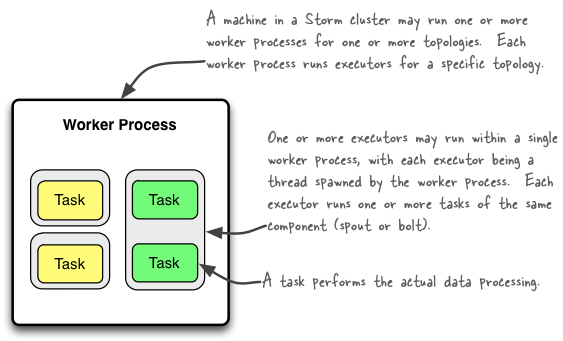
\includegraphics[width=\textwidth,natwidth=563,natheight=341]{img/relationships-worker-processes-executors-tasks.png}
    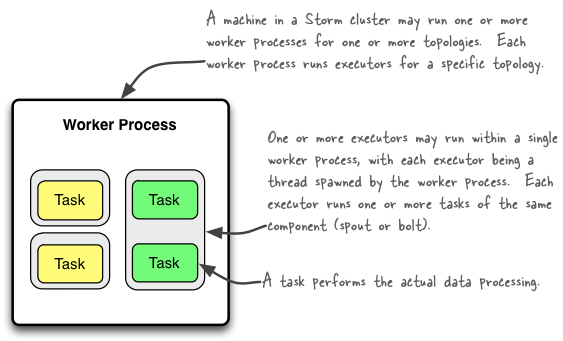
\includegraphics[scale=0.8]{img/relationships-worker-processes-executors-tasks.png}
    \caption{Storm Prozessschaubild\hspace{\linewidth}Bild von http://storm.apache.org/releases/1.1.1/Understanding-the-parallelism-of-a-Storm-topology.html}
  \end{figure}
\end{frame}


\subsection{Exactly-Once- / At-Least-Once-Semantik}
\begin{frame}[t]{Exactly-Once- / At-Least-Once-Semantik}
  Storm bietet „Guaranteed Message Processing“ $\Rightarrow$ allerdings mit
  At-Least-Once-Semantik
  \begin{itemize}
    \item Nachrichten werden auf jeden Fall verarbeitet
    \item im Fehlerfall wird die gleiche Nachricht nochmal gesendet
  \end{itemize}
  \pause
  Werden die Tuple nicht einzeln, sondern als (Micro-)Batch verarbeitet, so bietet Storm Trident
  \begin{itemize}
    \item Non-Transactional
    \item Transactional
    \item Opaque Transactional
  \end{itemize}
  Spouts. Damit ist eine Exactly-Once-Verarbeitung möglich.
\end{frame}

\subsection{Storm Trident}
\begin{frame}[t]{Storm Trident}
  Trident ist ein High-Level-Aufsatz auf Storm mit vorgefertigten Operationen:
  \begin{itemize}
    \item Merges / Joins
    \item Aggregationen (Count / Sum / Max)
    \item Gruppierungen
    \item Funktionen
    \item Filter
  \end{itemize}
  Trident verarbeitet keine einzelnen Tuple sondern „Micro-Batches“.
\end{frame}

\subsection{Powered By Storm}
\begin{frame}[t]{Powered By Storm}
  \begin{itemize}
    \item Groupon
    \item Twitter
    \item Yahoo!
    \item Spotify
    \item Alibaba
    \item Yelp
    \item PARC
  \end{itemize}
\end{frame}

\section{Word Count Beispiel}
\begin{frame}[t]{Word Count Beispiel}
  \begin{figure}
    \centering
    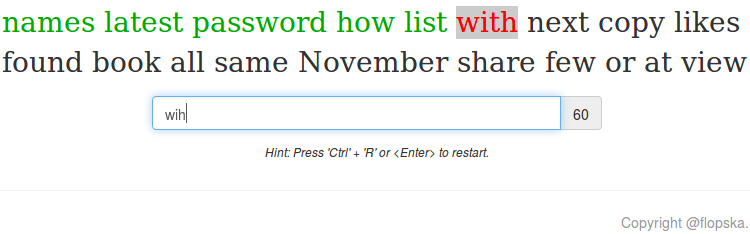
\includegraphics[scale=0.3,natwidth=750,natheight=234]{img/webapp.png}
    \caption{Erzeugen eines Wort-Streams\hspace{\linewidth}Screenshot von http://github.com/flopska/bigdatatools/}
  \end{figure}
\end{frame}

\begin{frame}[t]{Word Count Beispiel}
  \begin{figure}[h]
    \center
    \scalebox{.7}{\begin{tikzpicture}[>=stealth]
	\usetikzlibrary{shapes}
  \node (webapp)			at (0,2) [rectangle, draw, minimum height=1cm,thick,align=center] {Typing Webapp \\ {[.js]}};
  \node (kafka)			at (6,0) [rectangle split, rectangle split parts=8, rectangle split horizontal, draw, minimum height=1cm,thick,align=center,label=below:Kafka Message Queue] {};
  \node (kafka-rest)			at (6,2) [rectangle, draw, minimum height=1cm,thick] {kafka-rest};
  \node (confluent)			at (6,1) [rectangle, draw, minimum height=4.5cm,thick,text width=6cm,align=center,label=below:confluent] {};
  \node (storm)			at (12,0) [rectangle, draw, minimum height=1cm,thick,align=center] {Storm Topology\\ {[.java]}};

		\path
		(webapp)					edge[->,thick] (kafka-rest)
		(kafka-rest)					edge[->,thick] (kafka)
		(kafka)					edge[->,thick] (storm);
\end{tikzpicture}
}
    \caption{Architektur des Word Count Beispiels}
    \label{fig:wordcountsamplearchitecture}
  \end{figure}
\end{frame}

\begin{frame}[fragile]{Word Count Beispiel}
  \begin{lstlisting}
  public static void main(String[] args) {
    TridentTopology topology = new TridentTopology();
    BrokerHosts zk = new ZkHosts("localhost");
    TridentKafkaConfig spoutConf = new TridentKafkaConfig(zk, "words");
    spoutConf.scheme = new SchemeAsMultiScheme(new StringScheme());
    OpaqueTridentKafkaSpout spout = new OpaqueTridentKafkaSpout(spoutConf);
    WindowsStoreFactory mapState = new InMemoryWindowsStoreFactory();

    SlidingDurationWindow windowConfig = SlidingDurationWindow.of(
    new BaseWindowedBolt.Duration(10, TimeUnit.SECONDS),
    new BaseWindowedBolt.Duration(1, TimeUnit.SECONDS));
    topology.newStream("words", spout)
    .window(windowConfig, mapState, new Fields("str"), new CountAsAggregator(), new Fields("count"))
    .filter(new Debug());

    LocalCluster cluster = new LocalCluster("localhost", 2181L);
    cluster.submitTopology("localCluster2", new Config(), topology.build());
  }
  \end{lstlisting}
\end{frame}

\section{Literatur}
\begin{frame}[shrink=10]{Quellen}
  \begin{thebibliography}{Kleppmann, 2017}
      \setbeamertemplate{bibliography item}[book]
      \bibitem[Kleppmann, 2017]{Kleppmann2017}
      M.~Kleppmann.
      \newblock {\em Designing Data-Intensive Applications, 1st Edition}.
      \newblock O'Reilly Media, Inc., 2017

      \setbeamertemplate{bibliography item}[online]
      \bibitem[aufgerufen am 8. Dez 2017]{MicrosoftStreams}
      Microsoft
      \newblock {\em Was ist Stream Analytics?}.
      \newblock https://docs.microsoft.com/de-de/azure/stream-analytics/stream-analytics-introduction 

      \bibitem[aufgerufen am 8. Dez 2017]{MarzCAP}
      N.~Marz.
      \newblock {\em How to beat the CAP Theorem}.
      \newblock http://nathanmarz.com/blog/how-to-beat-the-cap-theorem.html 

      \bibitem[aufgerufen am 8. Dez 2017]{StormTutorial}
      Apache~Storm
      \newblock {\em Storm Tutorial}.
      \newblock http://storm.apache.org/releases/1.1.1/Tutorial.html 

      \bibitem[aufgerufen am 8. Dez 2017]{StormConcepts}
      Apache~Storm
      \newblock {\em Storm Concepts}.
      \newblock http://storm.apache.org/releases/1.1.1/Concepts.html

  \end{thebibliography}
\end{frame}

\end{document}
